% \section{Praktiken}

% \subsection{Fachpraxis}

\subsection{Application-Performance-Monitoring (APM)}

In der Praxis haben sich einige Technologien entwickelt und etabliert, welche die Nachvollziehbarkeit von Anwendungsverhalten und Nutzerinteraktion ermöglichen oder verbessern. Auf Basis der zuvor vorgestellten Methoden sowie neuer Ansätze haben sich in der Wirtschaft eine Reihe von Praktiken entwickelt. Einer dieser Ansätze ist das Application-Performance-Monitoring (APM, teils auch -Management).

Eine exakte Definition von APM lässt sich nicht nennen, denn es existiert kein Konsens, welche Eigenschaften und Funktionen ein APM umfasst. Ahmed \etal \cite{StudyingTheEffectivenessOfAPMTools}, Heger \etal \cite{APMStateOfTheArtAndChallenges}, Rabl \etal \cite{SolvingBigDataChallengesForAPM} sowie Dynatrace \cite{DynatraceAPM} definieren, dass ein APM eine Menge an Methoden, Techniken und Werkzeugen umfasst, die das System konstant überwachen und Aufschluss über den Zustand geben, sodass die Verfügbarkeit des Systems sichergestellt werden kann. Eine andere Definition vertreten Santos Filipe \cite{ClientSideMonitoringOfDistributedSystems}, New Relic \cite{NewRelicAPM} und Gartner \cite{GartnerMagicQuadrantForAPM}, welche APM weniger allgemeingültig, sondern über explizite Teilaspekte definieren, die es erfüllen muss, um als konformes APM bezeichnet zu werden. Aber auch innerhalb dieser Definition findet sich kein Konsens bzgl. der zu erfüllenden Aspekte, damit ein Monitoring-System zu einem APM wird.

In dieser Arbeit wird auf Basis der ersten und eher allgemeingültigen Definition ein APM definiert: Ein APM befasst sich mit dem Beobachten eines Softwaresystems und der Gewinnung von relevanten Daten aus diesem System zur näheren Analyse, um Rückschlüsse auf die Gesundheit des Systems zu ermöglichen und so die Verfügbarkeit sicherzustellen. Um dies zu erreichen, lassen sich 5 Fachgebiete einteilen, die unterschiedliche Aspekte eines Softwaresystems aufdecken \cite{ASurveyOfCloudMonitoringTools} \cite{GartnerMagicQuadrantForAPM} \cite{ResearchAndApplicationOfOperatingMonitoring}:

\begin{enumerate}
	\item Infrastruktur-Monitoring (IM)
	\item Application-and-Service-Monitoring (ASM)
	\item Real-User-Monitoring (RUM)
	\item Error-Monitoring
	\item Distributed-Tracing
\end{enumerate}

\subsubsection{Infrastructure-Monitoring (IM)}

Infrastructure-Monitoring beschäftigt sich hauptsächlich mit der Überwachung der Infrastruktur. Hierbei wird die Verfügbarkeit von Netzwerkressourcen sowie die Auslastung von Hard- und Softwareressourcen überwacht. Dieses Monitoring kann ohne Anpassungen der Software erfolgen und stellt somit ein Beispiel für Black-Box-Monitoring dar \cite{ClientSideMonitoringOfDistributedSystems}. Zum Beispiel ist die Überwachung von CPU- und Speicherausnutzung eines Systems ein Teil des Infrastructure-Monitoring.

\subsubsection{Application-and-Service-Monitoring (ASM)}

Bei Application-and-Service-Monitoring (ASM) handelt es sich um White-Box-Monitoring. Das bedeutet, dass die Softwarekomponenten angepasst werden müssen, sodass innerhalb der Laufzeitumgebungen Daten gesammelt werden können. Beispielsweise werden die Antwortzeit von Schnittstellaufrufen protokolliert und systematisch überwacht. Auf Basis der Daten lassen sich Abweichungen, von einzelnen Systemen oder vom aktuellen Gesamtsystem zu einem vorherigen Zeitpunkt feststellen.

\subsubsection{Real-User-Monitoring (RUM)}

\nomenclature[Fachbegriff]{UI}{User-Interface}

Real-User-Monitoring beschäftigt sich mit dem Mitschneiden von Nutzerinteraktionen und Umgebungseigenschaften einer Benutzeroberfläche \cite{IdentifyingWebPerformanceDegradations}. Um diese Daten zu ermitteln ist eine Änderung der Software für die Benutzeroberfläche notwendig, welches RUM zu einem White-Box-Monitoring macht. RUM wird jedoch nicht dazu verwendet, die Interaktionen eines einzelnen Nutzers aufzudecken, sondern Aufschluss über die gesamte Nutzerschaft der Anwendung zu erhalten. Die Daten werden oftmals nach den Interaktionen oder auch nach Umgebungseigenschaften, wie dem Browser der Nutzer gruppiert. Dadurch lassen sich Probleme bei der User-Experience \cite{AConceptLatticeForRecognitionOfUserProblems}, aber auch Performanceprobleme der Anwendung feststellen und sowie deren Ursache (z. B. die Umgebung des Nutzers) \cite{IdentifyingWebPerformanceDegradations}.

\subsubsection{Error-Monitoring}

Error-Monitoring konzentriert sich auf das Erfassen und Melden von Fehlern \cite{CrashbinCrashMonitoring}. Es lässt sich sowohl als White-Box- sowie als Black-Box-Monitoring umsetzen, da über existierende Protokollierung bereits Fehler festgestellt werden können. Hierzu kann es sinnvoll sein eine Software anzupassen, also White-Box-Monitoring einzusetzen, um mehr Kontextinformationen zu den Fehlern zu erfassen. Error-Monitoring wird oftmals eng mit Issue-Management verbunden, um aufgetretene Fehler und deren Behebung nachzuhalten \cite{CrashbinCrashMonitoring}.

\subsubsection{Distributed-Tracing}

Beim Distributed-Tracing handelt es sich um die fortgeschrittene Art des Tracings, welches systemübergreifend den Ablauf von Abfragen protokolliert (vgl. \autoref{sec:tracing}). Diese Art von Monitoring gibt, anders als die zuvor beschriebenen Arten, keine Einsicht in einzelne Komponenten, sondern veranschaulicht die resultierenden Interaktionen einer Abfrage.

\subsection{Log-Management}

Neben dem APM gibt es zudem weitere Funktionalitäten, wie z. B. das Log-Management, die Technologien in der Praxis vorweisen. Log-Management umfasst die Erfassung, Speicherung, Verarbeitung und Analyse von Logdaten von Anwendungen. Neben diesen Funktionen bieten solche Werkzeuge oftmals fundierte Suchfunktionen und Visualisierungsmöglichkeiten \cite{DesignLogManagementSystem}. Um die Daten aus einer Anwendung heraus zu exportieren, gibt es meist eine Vielzahl an Integrationen für Frameworks und Logbibliotheken.

Einer der wichtigsten Aspekte des Log-Managements, ist die Fähigkeit mit großen Datenmengen umzugehen und dabei den Nutzern zu ermöglichen auf diesen Daten zu arbeiten, Analysen durchzuführen und auch alte Datensätze abrufen zu können \cite{LoggingAndLogManagement}. Damit die teils enormen Datenmengen den Entwicklern und Betreibern zur Verfügung stehen, aber gleichzeitig nicht das System beeinträchtigen, sind spezielle Architekturkonzepte erforderlich. Beispielsweise werden selten abgerufene oder alte Daten in einen Langzeitspeicher überführt, welcher für die Speicherung optimiert ist, aber im Gegenzug keine zeitlich effizienten Ergebnisse liefern kann \cite{LoggingAndLogManagement}.

\subsection{Session-Replay}

Session-Replay beschreibt das Vorgehen, eine Sitzung eines Nutzers nachzustellen, so als ob sie gerade passiert \cite{NoBoundariesExfiltrationBySessionReplayScripts}. Hierbei können einzelne Aspekte der Anwendung nachgestellt werden, bspw. der Kommunikationsablauf oder die DOM-Manipulationen. Um eine realitätsnahe und entsprechend hilfreiche Nachstellung zu erstellen, sind viele Aspekte aufzuzeichnen. Ein realitätsnahes Session-Replay zeichnet eine enorme Datenmenge für jede Nutzersitzung auf und benötigt besonders beim Einsatz in Browsern eine effiziente Kommunikation, um die User-Experience (UX) nicht negativ zu beeinflussen \cite{AdvancedWebAnalyticsToolForMouseTracking} \cite{LogRocketPerformance}.

\begin{wrapfigure}[11]{r}{0.45\textwidth}
\vspace{-2.0\baselineskip}
\centering
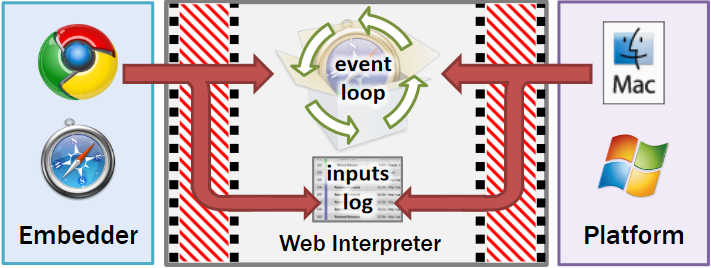
\includegraphics[width=\linewidth]{img/03_methoden/timelapse_figure5.png}
\caption{Mitschneiden von DOM-Events, Abb. aus \cite{TimelapsePaper}}
\label{fig:timelapse_figure5}
\smallskip\par
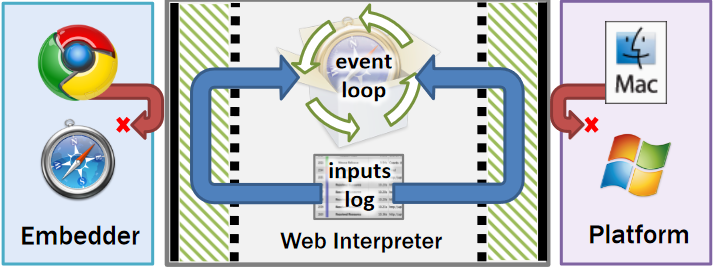
\includegraphics[width=\linewidth]{img/03_methoden/timelapse_figure6.png}
\caption{Abspielen von DOM-Events, Abb. aus \cite{TimelapsePaper}}
\label{fig:timelapse_figure6}
\end{wrapfigure}

Bereits 2013 entwickelten Burg \etal \cite{TimelapsePaper} mit \enquote{Timelapse} ein Framework, um Benutzersitzungen bei Webanwendungen aufzunehmen und wiederzugeben. Timelapse unterscheidet sich zu gängigen Session-Replay-Ansätzen dahingehend, dass die Wiedergabe keine vereinfachte Nachstellung der Anwendung ist. Stattdessen wird die JavaScript-Eventloop abgekapselt und es werden die Aufrufe von und zu der Eventloop mitgeschnitten (vgl. \autoref{fig:timelapse_figure5}).

Beim Abspielen werden die Aufrufe dann in derselben Reihenfolge an die Eventloop übergeben (vgl. \autoref{fig:timelapse_figure6}). Somit erfolgt eine exakte Wiederholung einer Sitzung, welches eine detaillierte Nachvollziehbarkeit ermöglicht. Leider benötigt dieser Ansatz eine gepatchte Version von WebKit \cite{WebKit}, weswegen auch Zugriff auf das System des Endnutzers vorausgesetzt wird. Zur Veröffentlichung des Berichtes bedeutete dies, dass die Browser Safari, Chrome und Opera unterstützt wurden - jedoch benutzt heute nur noch der Safari Webkit. Aufgrund der Notwendigkeit den Browser der Nutzer zu modifizieren und der Tatsache, dass es seit mehr als 5 Jahren\footnote{Timelapse GitHub Repo \url{https://github.com/burg/replay-staging/}} nicht mehr gepflegt wird, scheidet Timelapse für die hier angestrebte Lösung aus. Die vorgestellten Konzepte stellen jedoch nützliche Kernprinzipien für das Session Replay im Allgemeinen dar.